\documentclass[10pt,twocolumn]{article}

\usepackage[letterpaper,margin=0.70in,columnsep=0.24in]{geometry}
\usepackage[T1]{fontenc}
\usepackage[utf8]{inputenc}
\usepackage{times}
\usepackage{microtype}
\usepackage{graphicx}
\usepackage{booktabs}
\usepackage{amsmath,amssymb}
\usepackage{xcolor}
\usepackage{url}
\usepackage{hyperref}
\usepackage{caption}
\usepackage{enumitem}
\usepackage{balance}

\definecolor{xcyan}{HTML}{0891B2}
\definecolor{xnavy}{HTML}{0F172A}
\definecolor{xgray}{HTML}{475569}
\hypersetup{colorlinks=true,linkcolor=xcyan,citecolor=xcyan,urlcolor=xcyan,pdfauthor={Migel Tissera},pdftitle={Extending JPEG with neural networks (X-JPEG)}}
\captionsetup{font=small,labelfont=bf}
\setlength{\parindent}{1em}
\setlength{\parskip}{0pt}
\setlist{nosep,leftmargin=*}
\renewcommand{\topfraction}{0.95}
\renewcommand{\dbltopfraction}{0.95}
\renewcommand{\textfraction}{0.05}
\renewcommand{\floatpagefraction}{0.85}
\renewcommand{\dblfloatpagefraction}{0.85}

\newcommand{\xjpeg}{X-JPEG}
\newcommand{\msssim}{MS-SSIM}
\newcommand{\dqt}{DQT}

\begin{document}

\twocolumn[
\begin{center}
  {\LARGE\bfseries\color{xnavy} Extending JPEG with neural networks (X-JPEG):\\[3pt]
  Image-adaptive quantization with neural networks for JPEG\par}
  \vspace{0.7em}
  {\large Migel Tissera\par}
  \vspace{0.15em}
  {\normalsize Trinity Cloud\par}
  \vspace{0.35em}
  {\small Technical Report --- 4 August 2026\par}
  \vspace{0.25em}
  {\small\url{https://github.com/trinity-cloud/x-jpeg}\quad
   \url{https://huggingface.co/migtissera/x-jpeg}\par}
\end{center}
\vspace{0.35em}
\begin{minipage}{0.94\textwidth}
\begin{abstract}
JPEG is universally deployable because its bitstream and decoder are embedded in browsers, operating systems, cameras, content-delivery networks, and hardware. Its encoder, however, must decide how strongly to quantize each of 64 spatial-frequency coefficients in every color component. Conventional encoders begin with fixed, human-designed quantization-table shapes and expose a scalar quality control. We recast table selection as an image-conditioned prediction problem.

\xjpeg{} is an encoder-side neural extension that predicts three $8\!\times\!8$ quantization tables---one each for Y, Cb, and Cr---from the source image. A 2.20-million-parameter convolutional analysis transform combines a $256\!\times\!256$ image view with full-resolution DCT-band statistics. The predicted integer tables are passed to an ordinary JPEG encoder; the file is standards-compliant and needs no neural decoder. Training uses differentiable JPEG, exact-forward straight-through rounding, RGB \msssim{} with a luma guard, and a learned DCT-symbol rate proxy.

On 1,000 held-out COCO val2017 images at approximately 0.8 complete-file bits per pixel (bpp), the released three-table model reaches 0.97322 RGB \msssim{}. It exceeds its fixed-average-table control by 0.000444 (paired 95\% bootstrap CI 0.000168--0.000731) and its shuffled-table control by 0.001427 (0.000997--0.001844), establishing that image/table assignment contributes to quality. A two-emitted-table path reaches 0.97345 versus 0.97282 for jpegli at nearly identical rate, while jpegli remains better on luma-only \msssim{}. An exploratory 100-image native study improves over Annex-K tables under the same MozJPEG backend by 0.00355 RGB \msssim{} near 0.5 bpp and 0.00527 near 0.25 bpp; WebP remains strongest in the 0.25-bpp pilot.
\end{abstract}
\end{minipage}
\vspace{0.9em}
]

\section{Introduction}

Learned image compression has produced strong rate--distortion results, but most learned codecs replace the bitstream, the decoder, or both. That trade is difficult across the open web, where JPEG's accumulated compatibility is itself a product feature.

This work starts from a different constraint: \emph{the decoder and file format remain ordinary JPEG}. A neural network may spend computation while encoding, but it must leave behind only information a standard decoder already understands. Quantization tables are an unusually attractive intervention point. They are explicit encoder decisions, carried in Define Quantization Table (DQT) segments, and consumed by every conforming decoder~\cite{itu1992jpeg,wallace1992jpeg}.

Traditional quantization tables are fixed frequency-shaping priors. A quality setting normally scales those priors but does not reconsider their shape for the image. Yet portraits, foliage, illustrations, and night photographs distribute energy and perceptual importance differently across frequency and color. \xjpeg{} asks whether a network can predict a better table shape for every image without changing JPEG syntax.

Predicted variation alone is insufficient. A model can collapse to one global table or emit arbitrary image-dependent variation hidden by later operating-point search. We define \emph{useful adaptivity} causally: the correctly paired image/table must beat both a dataset-average predicted table and wrong-image tables under common rate control. The released model passes both controls on 1,000 held-out images.

Our contributions are:
\begin{enumerate}
  \item an encoder-only neural extension that predicts image-specific standard JPEG tables;
  \item a compact three-table architecture combining a thumbnail with frequency-aligned full-resolution DCT statistics;
  \item a JPEG-aware training graph with straight-through quantization, perceptual distortion, learned rate estimation, and optional table-entropy/autoencoder regularizers;
  \item a complete-file evaluation with fixed-average and shuffled-table adaptivity controls; and
  \item open source, released weights, pinned backends, and cross-platform Python wheels.
\end{enumerate}

This report concerns the independently trained 2026 release. It does not report results from or distribute weights belonging to the earlier private implementation that motivated the reconstruction.

\begin{figure*}[t]
  \centering
  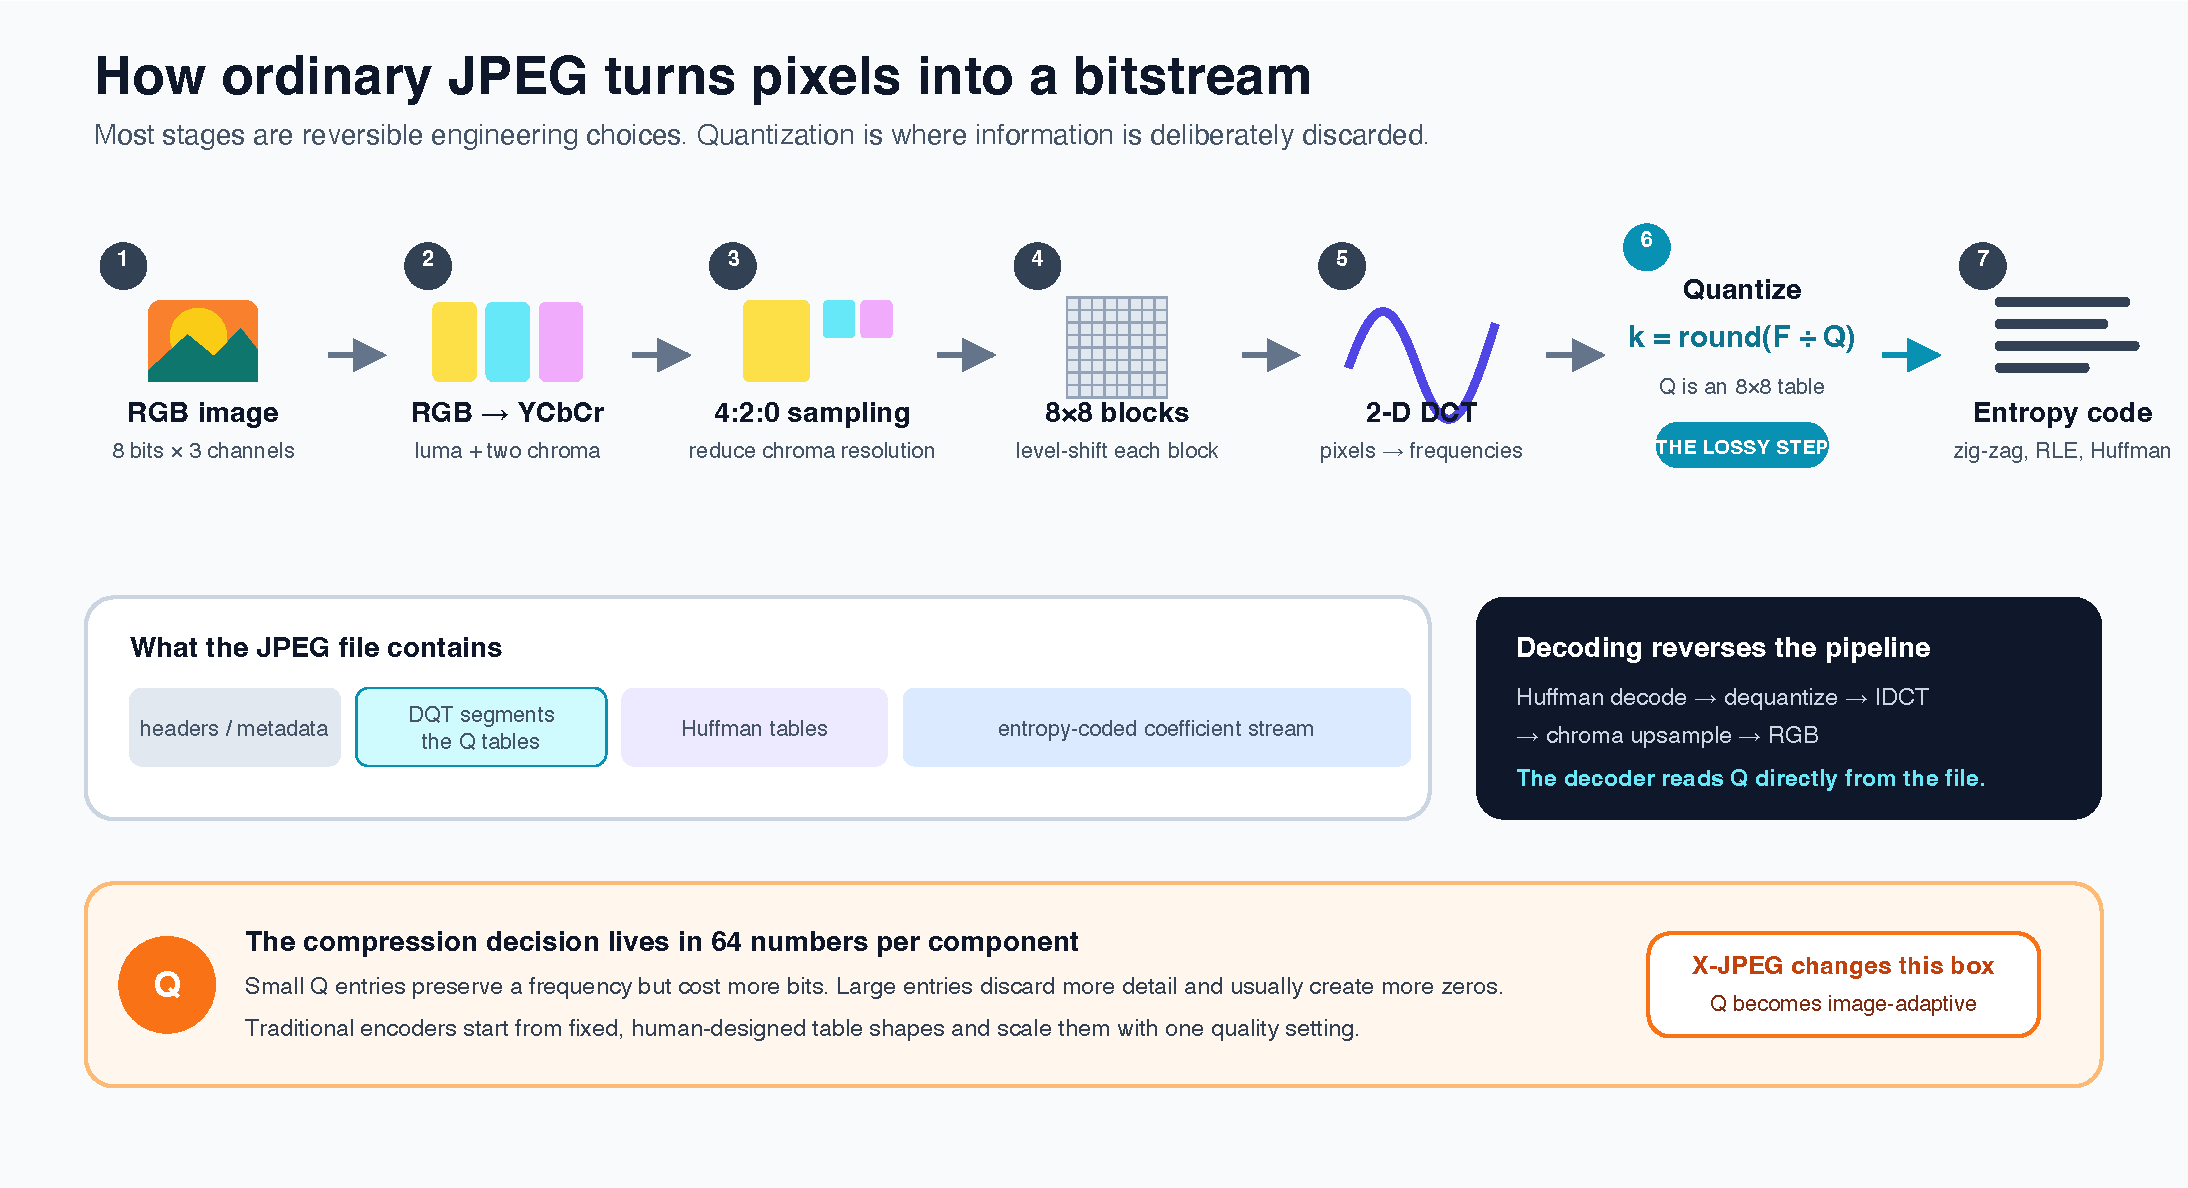
\includegraphics[width=\textwidth]{figures/pdf/01-jpeg-pipeline.pdf}
  \caption{Baseline JPEG encoding. Quantization is the central lossy decision. Q tables are written into the file, so changing how an encoder selects them does not require a new decoder.}
  \label{fig:jpeg}
\end{figure*}

\section{JPEG as an optimization problem}

\subsection{Baseline pipeline}

JPEG commonly transforms RGB into one luma and two chroma components, subsamples chroma, level-shifts samples, and divides each component into non-overlapping $8\!\times\!8$ blocks~\cite{itu1992jpeg,wallace1992jpeg}. For a block $B$, the two-dimensional DCT is
\begin{equation}
  F = D B D^\top,
\end{equation}
where $D$ is the orthonormal eight-point DCT matrix. Given component table $Q$, the encoder transmits
\begin{equation}
  K_{u,v}=\operatorname{round}\!\left(F_{u,v}/Q_{u,v}\right).
\end{equation}
The decoder reconstructs $\hat F=K\odot Q$, applies the inverse DCT, upsamples chroma, and converts to RGB. Zig-zag ordering, run-length coding, DC prediction, and Huffman coding compress the symbols without additional distortion.

Small $Q$ entries preserve a frequency more accurately but usually require more bits; large entries discard more information and produce more zeros. Because JPEG transmits $Q$, the tables are encoder policy rather than immutable decoder behavior (Fig.~\ref{fig:jpeg}).

\subsection{Scope of adaptivity}

\xjpeg{} predicts one table set per image. The tables are global within each image and component. This is image-adaptive, not block-adaptive: all luma blocks share the Y table. This choice preserves ordinary JPEG syntax but cannot perform the spatial allocation available to formats with segmentation or block-level controls, such as lossy WebP~\cite{webp}.

\subsection{Rate definition}

Every reported rate is computed from the complete file,
\begin{equation}
  \mathrm{bpp}=\frac{8\,|\text{encoded file in bytes}|}{HW}.
\end{equation}
The numerator includes headers, DQT payloads, Huffman tables, scan headers, and entropy-coded data. We do not divide by three color channels. Thus 0.8 bpp means 0.8 compressed bits per RGB pixel location, compared with 24 uncompressed bits for 8-bit RGB.

\section{Related work}

Ball\'e, Laparra, and Simoncelli introduced end-to-end learned analysis/synthesis transforms with generalized divisive normalization (GDN) and continuous quantization relaxations~\cite{balle2016gdn,balle2017compression}. Hyperpriors later improved entropy estimates through learned side information~\cite{balle2018hyperprior}. These systems established the power of learned nonlinear transforms, but generally require a custom decoder and bitstream.

Straight-through estimators provide gradient surrogates for hard operations~\cite{bengio2013ste}. Differentiable JPEG implementations approximate the codec; Reich et al. show that color conversion, subsampling, rounding, and boundary conventions materially affect fidelity to a real implementation~\cite{reich2024diffjpeg}. We use a differentiable training model but re-encode every reported point with a real codec.

DeepN-JPEG and related table optimization target neural-network classification rather than human-perceptual reconstruction~\cite{liu2018deepnjpeg,li2020optjpeg}. Neural JPEG jointly learns frequency-domain pre/post-editing and quantization tables, placing learned processing at both encoder and decoder~\cite{mali2022neuraljpeg}. \xjpeg{} occupies a narrower compatibility point: deployed neural computation selects only standard DQT values. There is no learned prefilter a decoder must reverse and no learned post-processing after decode.

\begin{figure*}[t]
  \centering
  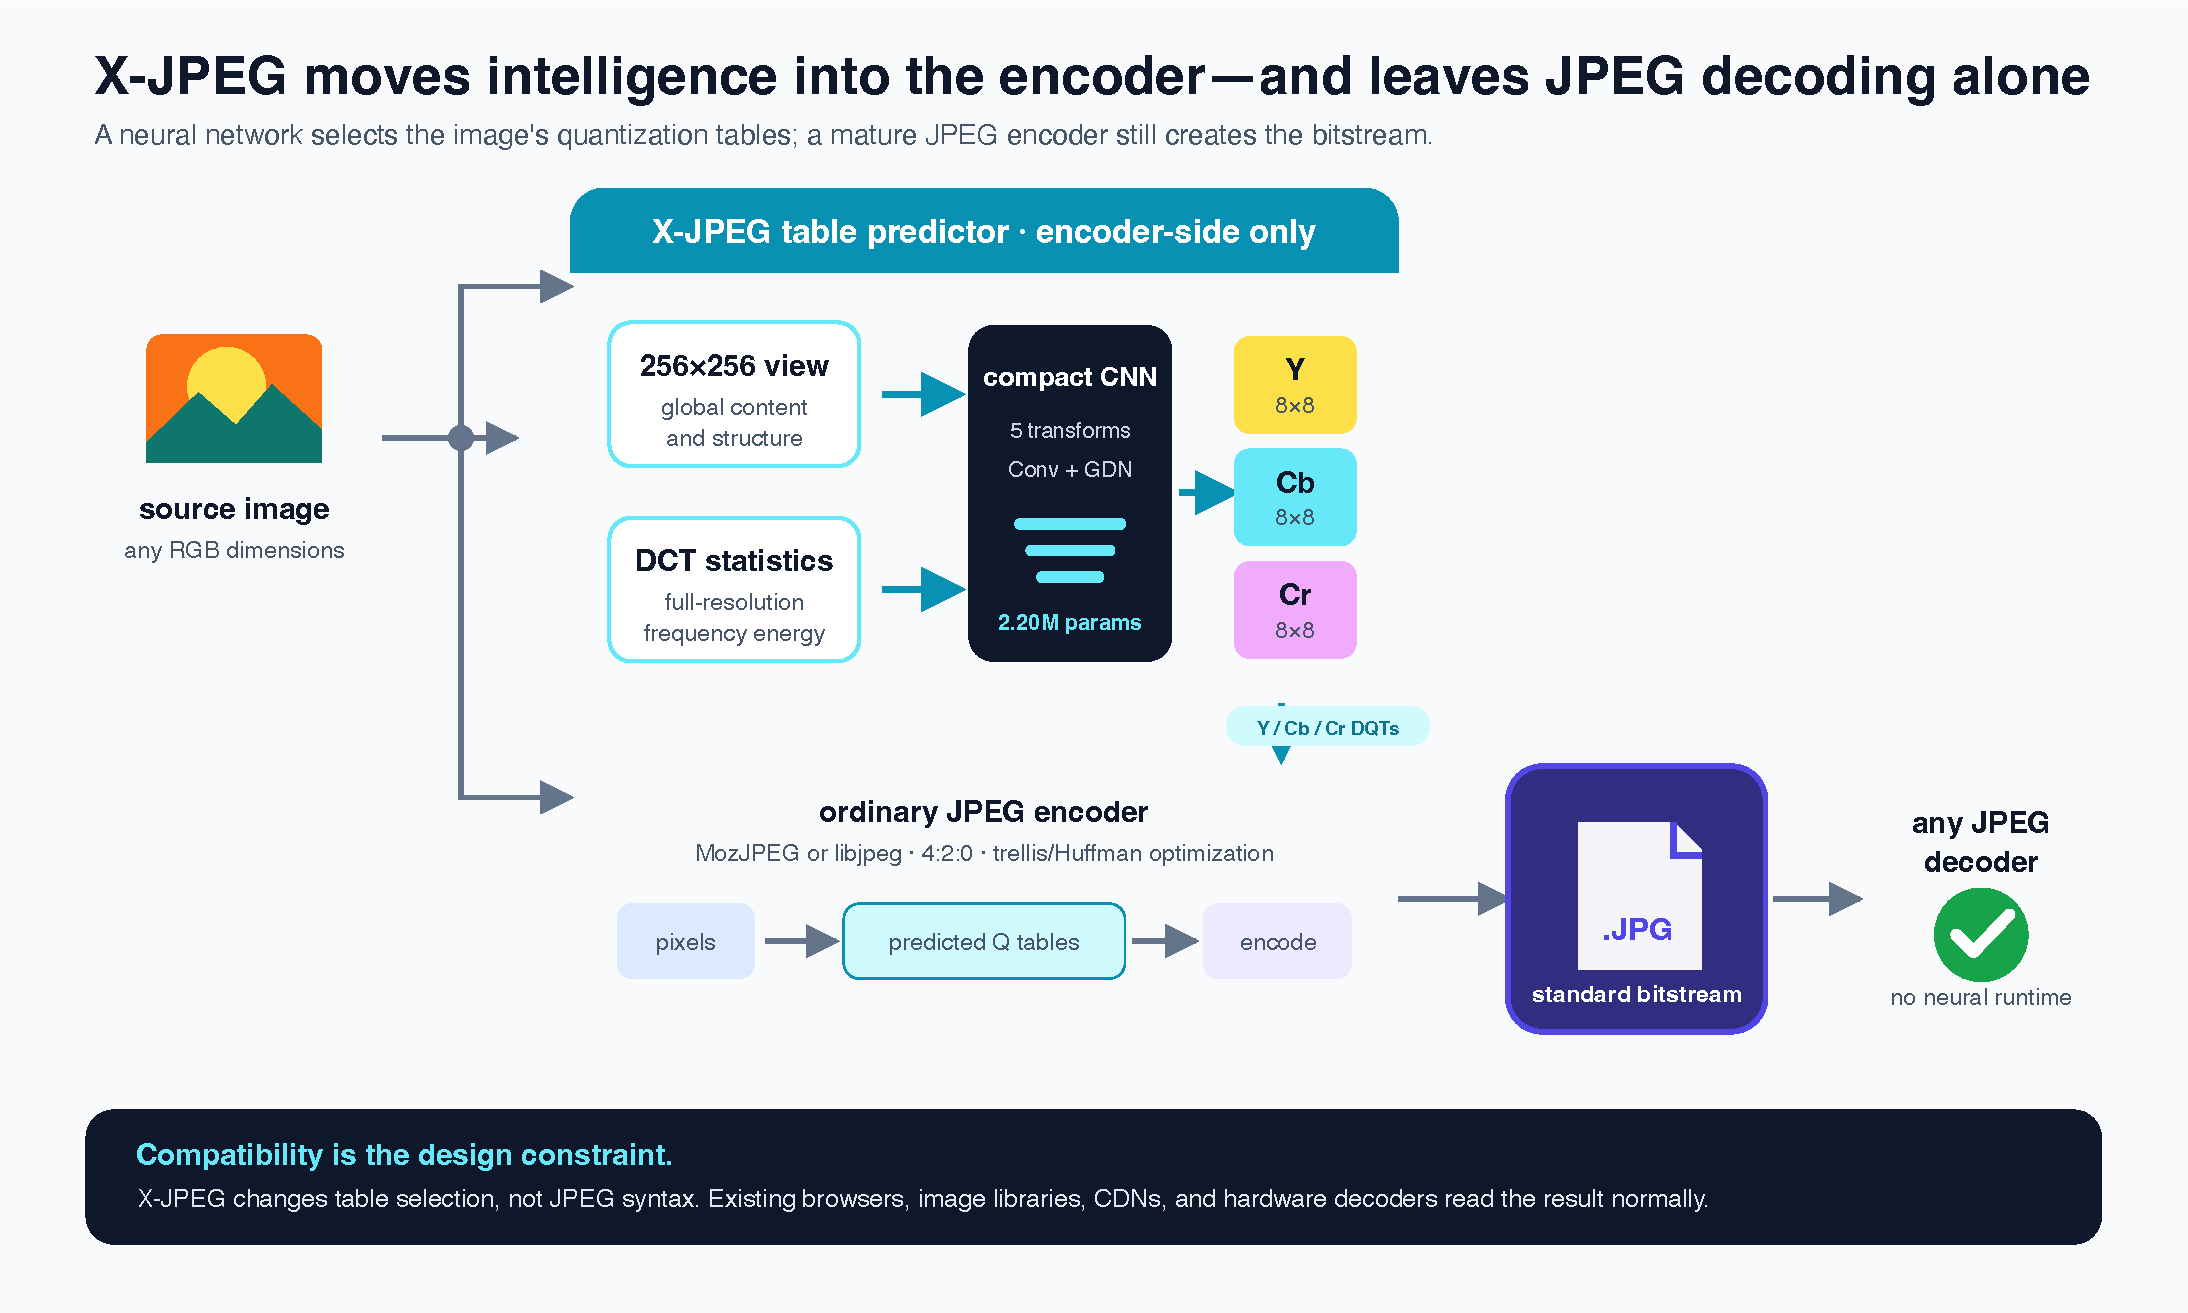
\includegraphics[width=\textwidth]{figures/pdf/02-xjpeg-integration.pdf}
  \caption{\xjpeg{} deployment boundary. Source pixels and predicted tables enter a mature JPEG encoder. The output is a normal JPEG; no model is required to decode it.}
  \label{fig:integration}
\end{figure*}

\section{Method}

\subsection{Image-conditioned table prediction}

For RGB image $x$, the network predicts
\begin{equation}
 T_\theta(x)=\left(Q^Y,Q^{Cb},Q^{Cr}\right),\quad
 Q^c\in\{1,\ldots,255\}^{8\times8}.
\end{equation}
It receives two complementary views: a bicubic $256\!\times\!256$ RGB thumbnail for global content, and a $3\!\times\!8\!\times\!8$ tensor of full-resolution log DCT-band energy. The latter retains frequency evidence that thumbnailing can erase.

Four $5\!\times\!5$, stride-2 convolution + reparameterized GDN blocks with widths 64, 128, 192, and 256 map spatial dimensions $256\!\rightarrow\!128\!\rightarrow\!64\!\rightarrow\!32\!\rightarrow\!16$. A final $5\!\times\!5$, stride-2 convolution emits $3\!\times\!8\!\times\!8$ raw codes. Each full-resolution statistic is added to the matching component/frequency code with a learned scalar gain, avoiding convolution across unrelated DCT bands.

Raw codes map to legal table values via
\begin{equation}
  T(z)=1+254\,\sigma(z/4).
\end{equation}
Training can add $\mathcal U(-\tfrac12,\tfrac12)$ noise before the table-entropy model; inference rounds and clamps to $[1,255]$. The released encoder contains 2,196,355 parameters.

\begin{figure*}[t]
  \centering
  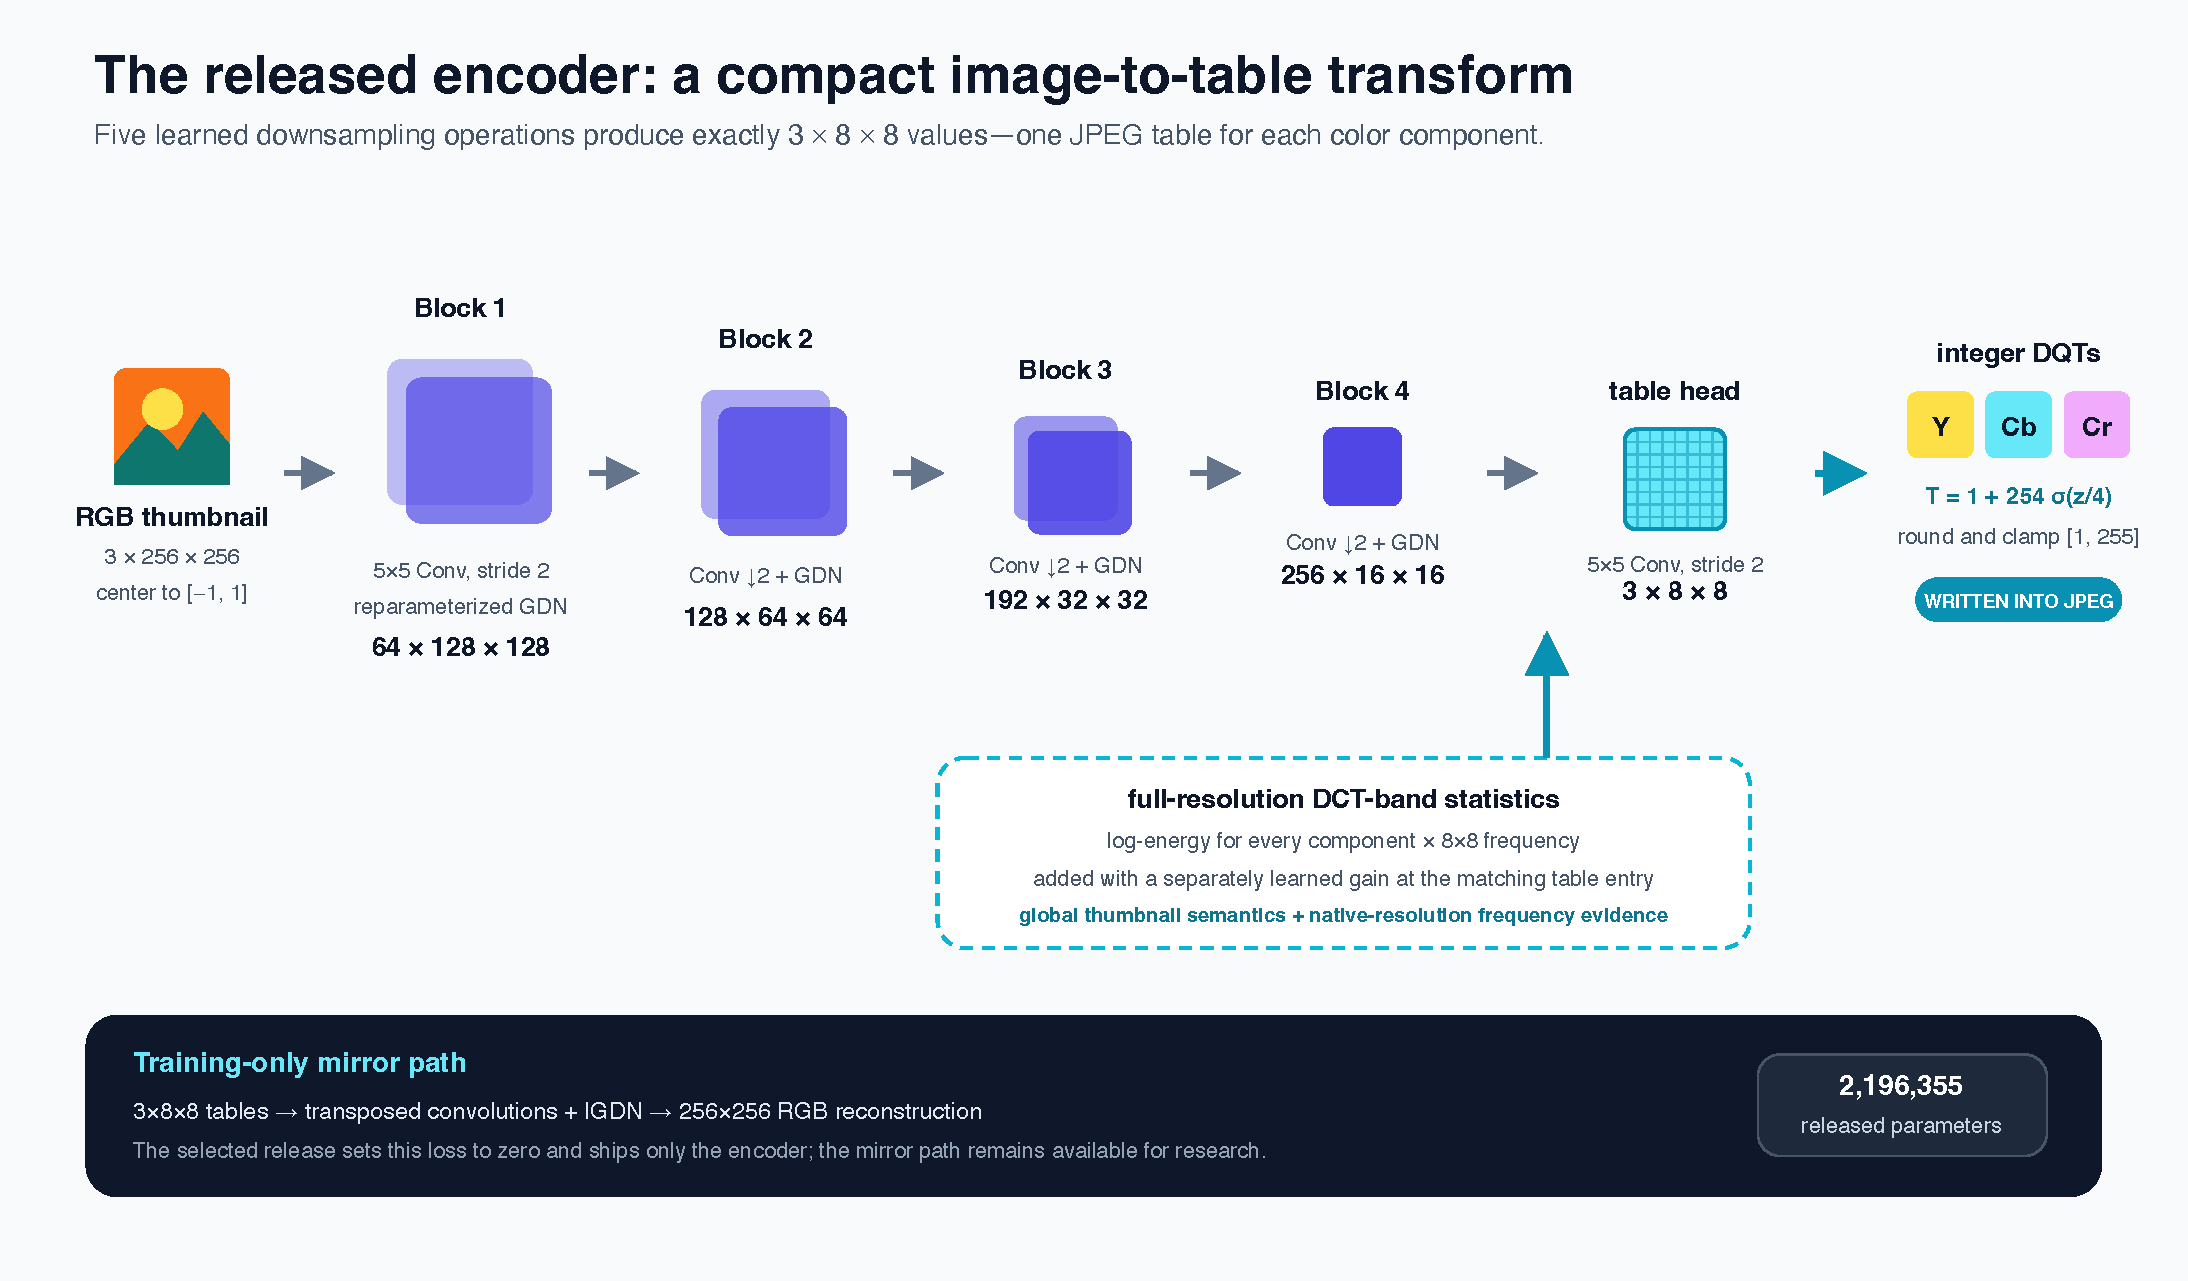
\includegraphics[width=\textwidth]{figures/pdf/03-network-architecture.pdf}
  \caption{Released compact encoder. A mirror transposed-convolution/IGDN decoder is training-only and is absent from the inference artifact.}
  \label{fig:architecture}
\end{figure*}

\subsection{Three predictions, two emission modes}

The network predicts independent Y, Cb, and Cr tables. JPEG can emit all three. For small files, however, a third DQT costs roughly 65 bytes. The default product path averages the two predicted chroma tables at the encoding boundary and emits Y plus shared chroma. The three-output predictor remains unchanged. Three DQTs provide the clean adaptivity experiment; two emitted DQTs often provide the better small-file product trade-off.

\subsection{Differentiable JPEG}

The training codec implements RGB $\rightarrow$ YCbCr $\rightarrow$ 4:2:0 $\rightarrow$ block DCT $\rightarrow$ table division $\rightarrow$ quantization and the inverse path. For $s=F/Q$, straight-through rounding is
\begin{equation}
 \operatorname{STEround}(s)=s+\operatorname{stopgrad}(\operatorname{round}(s)-s).
\end{equation}
The forward value is exact integer rounding and the surrogate backward derivative is one. This prevents the predictor from exploiting fractional signal a real JPEG would discard.

\subsection{Objective}

The training family uses
\begin{align}
\mathcal D={}&1-\operatorname{MS\!\text{-}\!SSIM}_{RGB} \nonumber\\
 &+\lambda_L\big(1-\operatorname{MS\!\text{-}\!SSIM}_{Y}\big),\\
\mathcal L={}&\lambda_d\mathcal D+\lambda_r R_{DCT}+\lambda_T R_{table} \nonumber\\
 &+\lambda_{AE}\mathcal L_{AE}+\lambda_{MSE}\mathcal L_{MSE}.
\end{align}
The released continuation uses $\lambda_d=1$, $\lambda_L=0.25$, $\lambda_r=0.05$, and zero final weights for table entropy, mirror reconstruction, and JPEG MSE.

For each component and frequency, a learned Laplace density estimates quantized coefficient mass,
\begin{equation}
R_{DCT}=-\sum_i\log_2 P_\phi(k_i-\tfrac12<K_i<k_i+\tfrac12).
\end{equation}
This omits exact DC differencing, run symbols, categories, optimized Huffman lengths, and headers. It is a gradient, not reported bitrate.

A Ball\'e-style factorized density can similarly estimate soft table entropy $R_{table}$. Since DQT entries are stored literally, this is a regularizer rather than a file-size saving. Ablation selected $\lambda_T=0$. A mirror IGDN decoder can reconstruct the thumbnail from the table bottleneck, encouraging early image conditioning; it is optional, has zero weight in the selected continuation, and is not shipped.

\begin{figure*}[t]
  \centering
  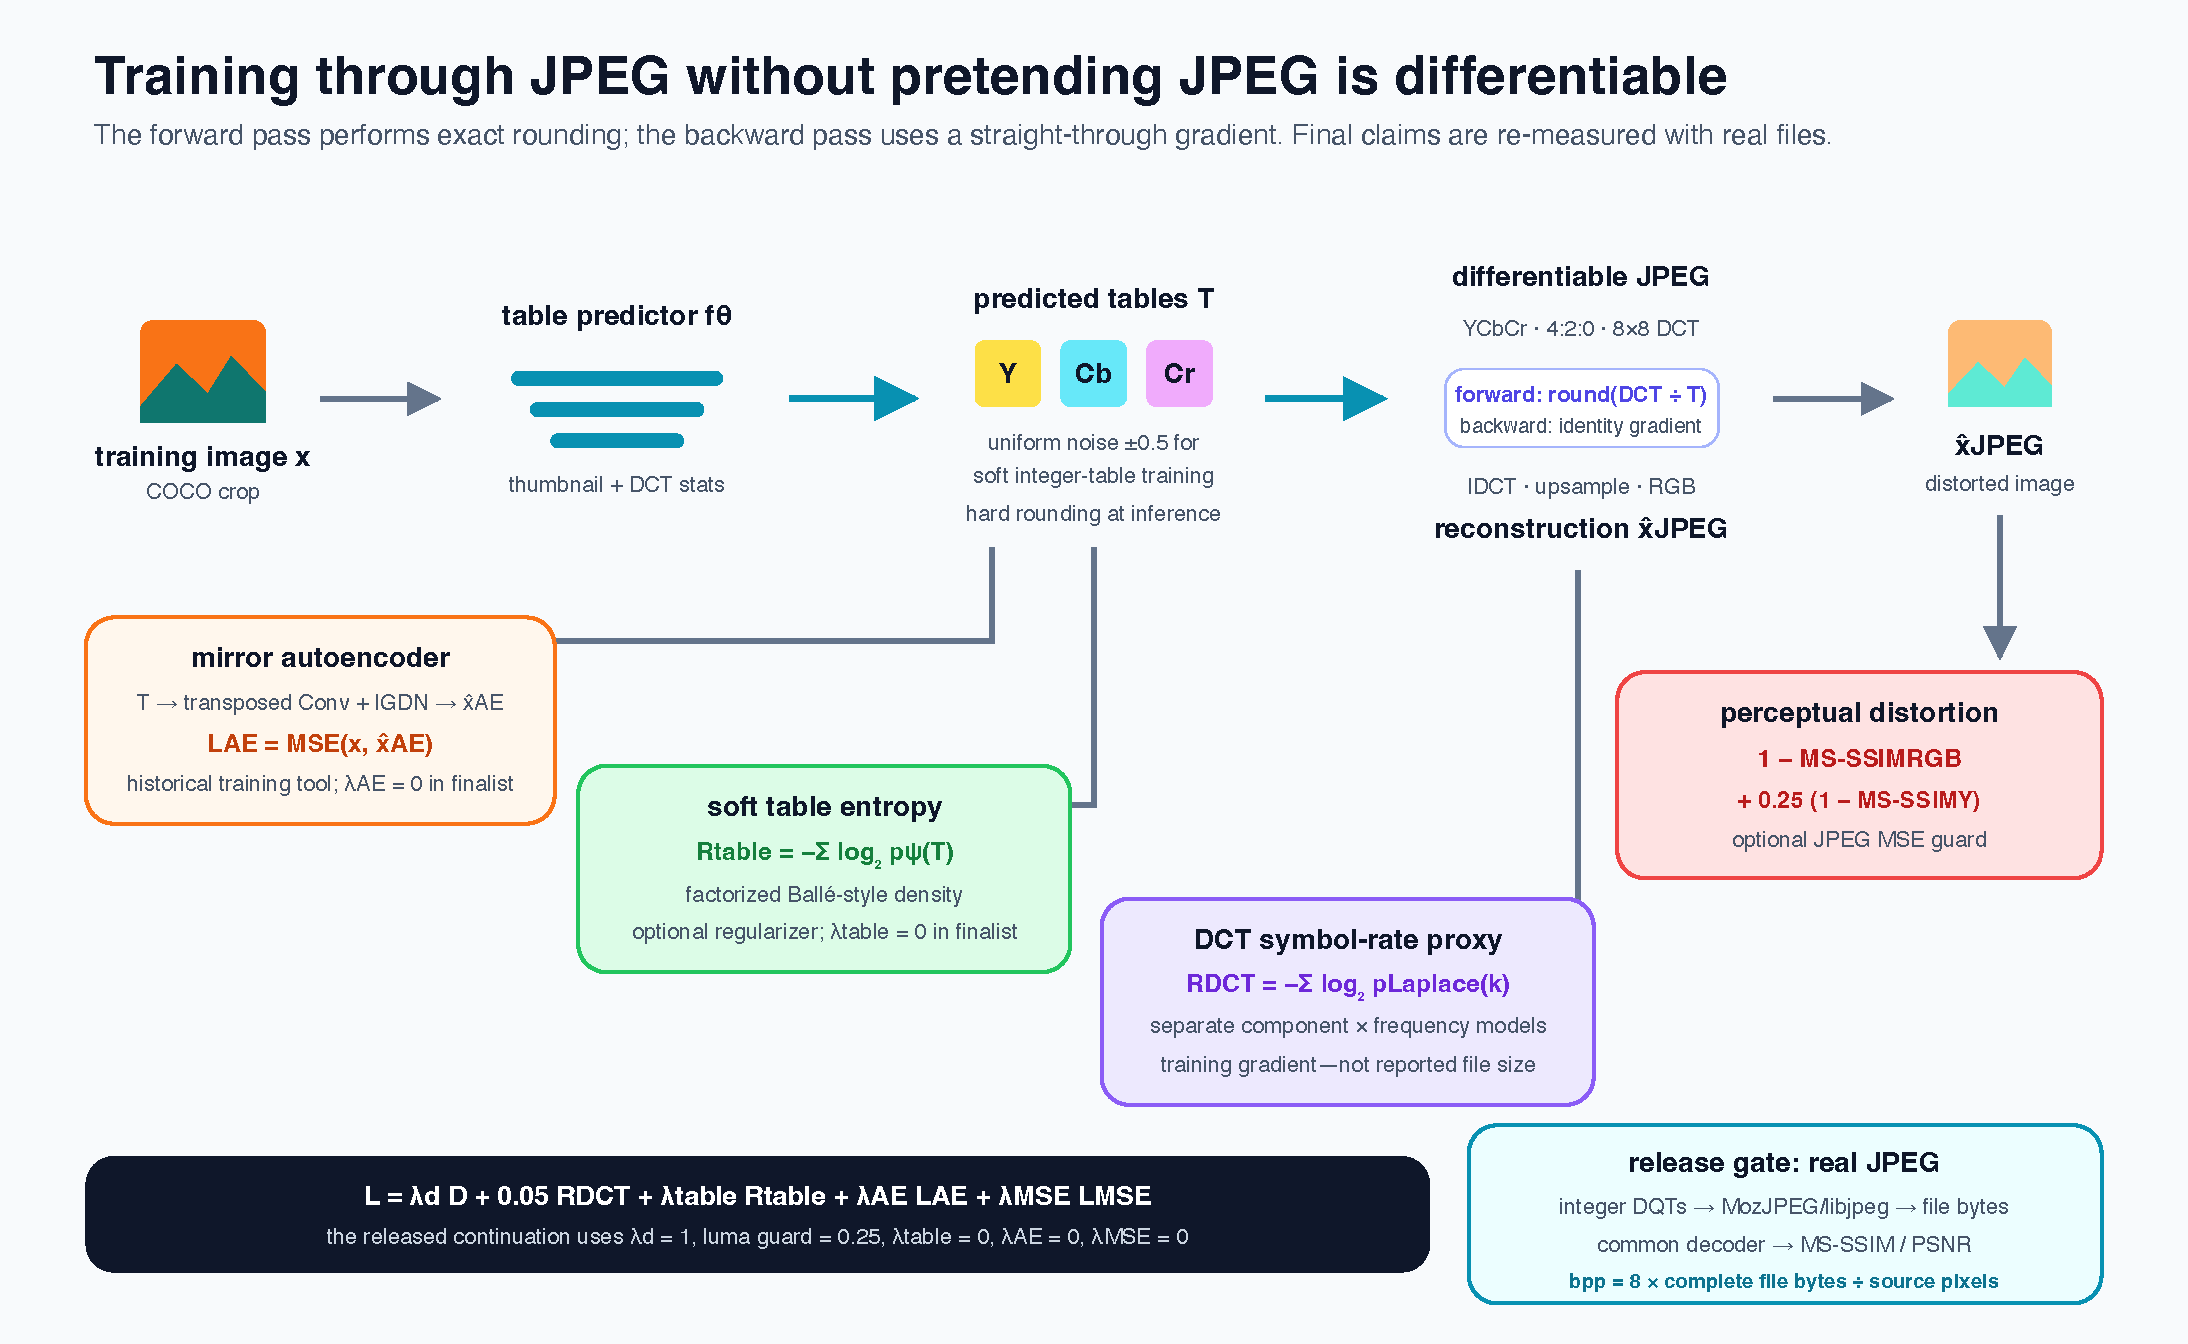
\includegraphics[width=\textwidth]{figures/pdf/04-training-objective.pdf}
  \caption{Training graph and release gate. Proxy losses enable optimization; a real encoder, complete file size, and common decoder determine release metrics.}
  \label{fig:training}
\end{figure*}

\subsection{Real encoding and rate control}

At deployment, tables are multiplied by scalar $s$, rounded, clamped, and passed to MozJPEG or libjpeg. The public API can search $s$ per image for a target rate or minimum RGB \msssim{}. Scientific adaptivity tests instead use one dataset-wide scalar so rate search cannot compensate for a wrong table.

Official wheels bundle pinned MozJPEG. MozJPEG retains JPEG compatibility while adding trellis quantization, optimized Huffman coding, progressive scan optimization, and perceptual presets~\cite{mozjpeg}. \xjpeg{} proposes table shape; MozJPEG efficiently codes coefficients under it.

\section{Experiments}

\subsection{Training and protocol}

The release model was trained on COCO train2017~\cite{lin2014coco} using random $256\!\times\!256$ crops. The final product lineage adds frequency statistics and a 0.25 luma guard in a 2,500-step stage followed by a 5,000-step continuation (batch 96, model learning rate $10^{-4}$, rate-model learning rate $10^{-3}$), initialized from an earlier RGB/rate model.

Evaluation uses held-out COCO val2017 in a controlled 256 domain and at native resolution. All encoders receive identical lossless pixels, use 4:2:0, one dataset-wide operating parameter, and a common Pillow/libjpeg decode. We report full-file bpp, canonical five-scale RGB \msssim{}~\cite{wang2003msssim}, luma \msssim{}, 6:1:1 Y:Cb:Cr \msssim{}, and RGB PSNR.

The high-power study uses 1,000 images. The exploratory low-rate study uses 100 native images and compares \xjpeg{}+MozJPEG, Annex-K+the same MozJPEG, MozJPEG's MS-SSIM mode, and WebP method 6. MozJPEG is pinned at \texttt{0826579...1437}; jpegli at \texttt{031a007...5620}~\cite{jpegli}.

\subsection{High-power result near 0.8 bpp}

\begin{table*}[t]
\centering
\caption{COCO-val-1000, controlled 256 domain. Complete-file rate; best in bold.}
\label{tab:highpower}
\small
\begin{tabular}{lccccc}
\toprule
Encoder & bpp $\downarrow$ & RGB \msssim{} $\uparrow$ & Y \msssim{} $\uparrow$ & 6:1:1 $\uparrow$ & PSNR $\uparrow$ \\
\midrule
libjpeg-turbo / Annex-K & 0.7979 & 0.96874 & \textbf{0.98592} & 0.97682 & 29.00 \\
\xjpeg{}, three emitted DQTs & 0.7985 & 0.97322 & 0.98269 & 0.98017 & 29.44 \\
\textbf{\xjpeg{}, shared emitted chroma} & \textbf{0.7981} & \textbf{0.97345} & 0.98305 & \textbf{0.98047} & \textbf{29.50} \\
jpegli & 0.7986 & 0.97282 & 0.98572 & 0.97935 & 29.26 \\
\bottomrule
\end{tabular}
\end{table*}

The shared-chroma path exceeds jpegli by 0.000628 paired RGB \msssim{} (95\% bootstrap CI 0.000389--0.000871) while using 0.00050 fewer bpp. It gains 0.00111 in 6:1:1 \msssim{} and 0.23 dB RGB PSNR. This is not a universal quality win: jpegli is 0.00267 higher on luma-only \msssim{}.

On native COCO-val-1000, three-DQT \xjpeg{} reaches 0.79981 bpp / 0.97022 RGB \msssim{} versus jpegli at 0.79985 / 0.96892. The paired difference is 0.001299 (95\% CI 0.000970--0.001635). \xjpeg{} gains 0.00096 in 6:1:1 and 0.11 dB RGB PSNR; jpegli is 0.00221 higher on luma.

\subsection{Does the network use the image?}

Across the 1,000-image set, table entries have mean standard deviation 7.923, or 21.266\% relative variation. Variation alone does not prove utility. Table~\ref{tab:adaptive} compares correct assignment, the fixed dataset-average table, cyclically shuffled tables, and Annex-K under one scalar per method.

\begin{table}[t]
\centering
\caption{Adaptivity controls at $\approx$0.8 bpp, $n=1000$.}
\label{tab:adaptive}
\small
\resizebox{\columnwidth}{!}{%
\begin{tabular}{lcccc}
\toprule
Method & bpp & RGB MS & Y MS & PSNR \\
\midrule
adaptive \xjpeg{} & 0.7985 & \textbf{0.97322} & 0.98269 & \textbf{29.44} \\
fixed average & 0.7984 & 0.97278 & 0.98233 & 29.35 \\
shuffled & 0.7987 & 0.97180 & 0.98150 & 29.29 \\
Annex-K & 0.7989 & 0.96885 & \textbf{0.98594} & 29.01 \\
\bottomrule
\end{tabular}}
\end{table}

Adaptive minus fixed is +0.000444 RGB \msssim{} (95\% CI +0.000168 to +0.000731); adaptive minus shuffled is +0.001427 (+0.000997 to +0.001844). Both intervals exclude zero. The predictor therefore contributes more than a learned global table: matching a table to its image matters.

\subsection{Exploratory low-rate behavior}

\begin{table*}[t]
\centering
\caption{Native COCO-val-100 exploratory low-rate aggregate. The study lacks paired intervals.}
\label{tab:lowrate}
\small
\begin{tabular}{lcccc}
\toprule
 & \multicolumn{2}{c}{0.5-bpp target} & \multicolumn{2}{c}{0.25-bpp target} \\
Encoder & bpp & RGB \msssim{} & bpp & RGB \msssim{} \\
\midrule
\xjpeg{}, 2 DQT + MozJPEG & 0.49975 & 0.95718 & 0.25111 & 0.91764 \\
\xjpeg{}, 3 DQT + MozJPEG & 0.49917 & 0.95693 & 0.25002 & 0.91642 \\
Annex-K + MozJPEG & 0.50097 & 0.95363 & 0.25000 & 0.91237 \\
MozJPEG MS-SSIM & 0.50618 & \textbf{0.95759} & 0.24472 & 0.91495 \\
WebP method 6 & 0.50015 & 0.95668 & 0.24996 & \textbf{0.92252} \\
\bottomrule
\end{tabular}
\end{table*}

At 0.5 bpp, two-DQT \xjpeg{} is +0.00355 RGB \msssim{} over Annex-K under the same MozJPEG backend, +0.00050 over WebP, and $-0.00041$ below the tuned MozJPEG point (whose rate is 0.00643 bpp higher). At 0.25 bpp, \xjpeg{} is +0.00527 over Annex-K and +0.00268 over the measured MozJPEG point, but WebP is +0.00488 ahead. The gain over a fixed JPEG table grows under the tighter budget, but this 100-image aggregate motivates rather than settles the low-rate comparison.

\begin{figure*}[t]
  \centering
  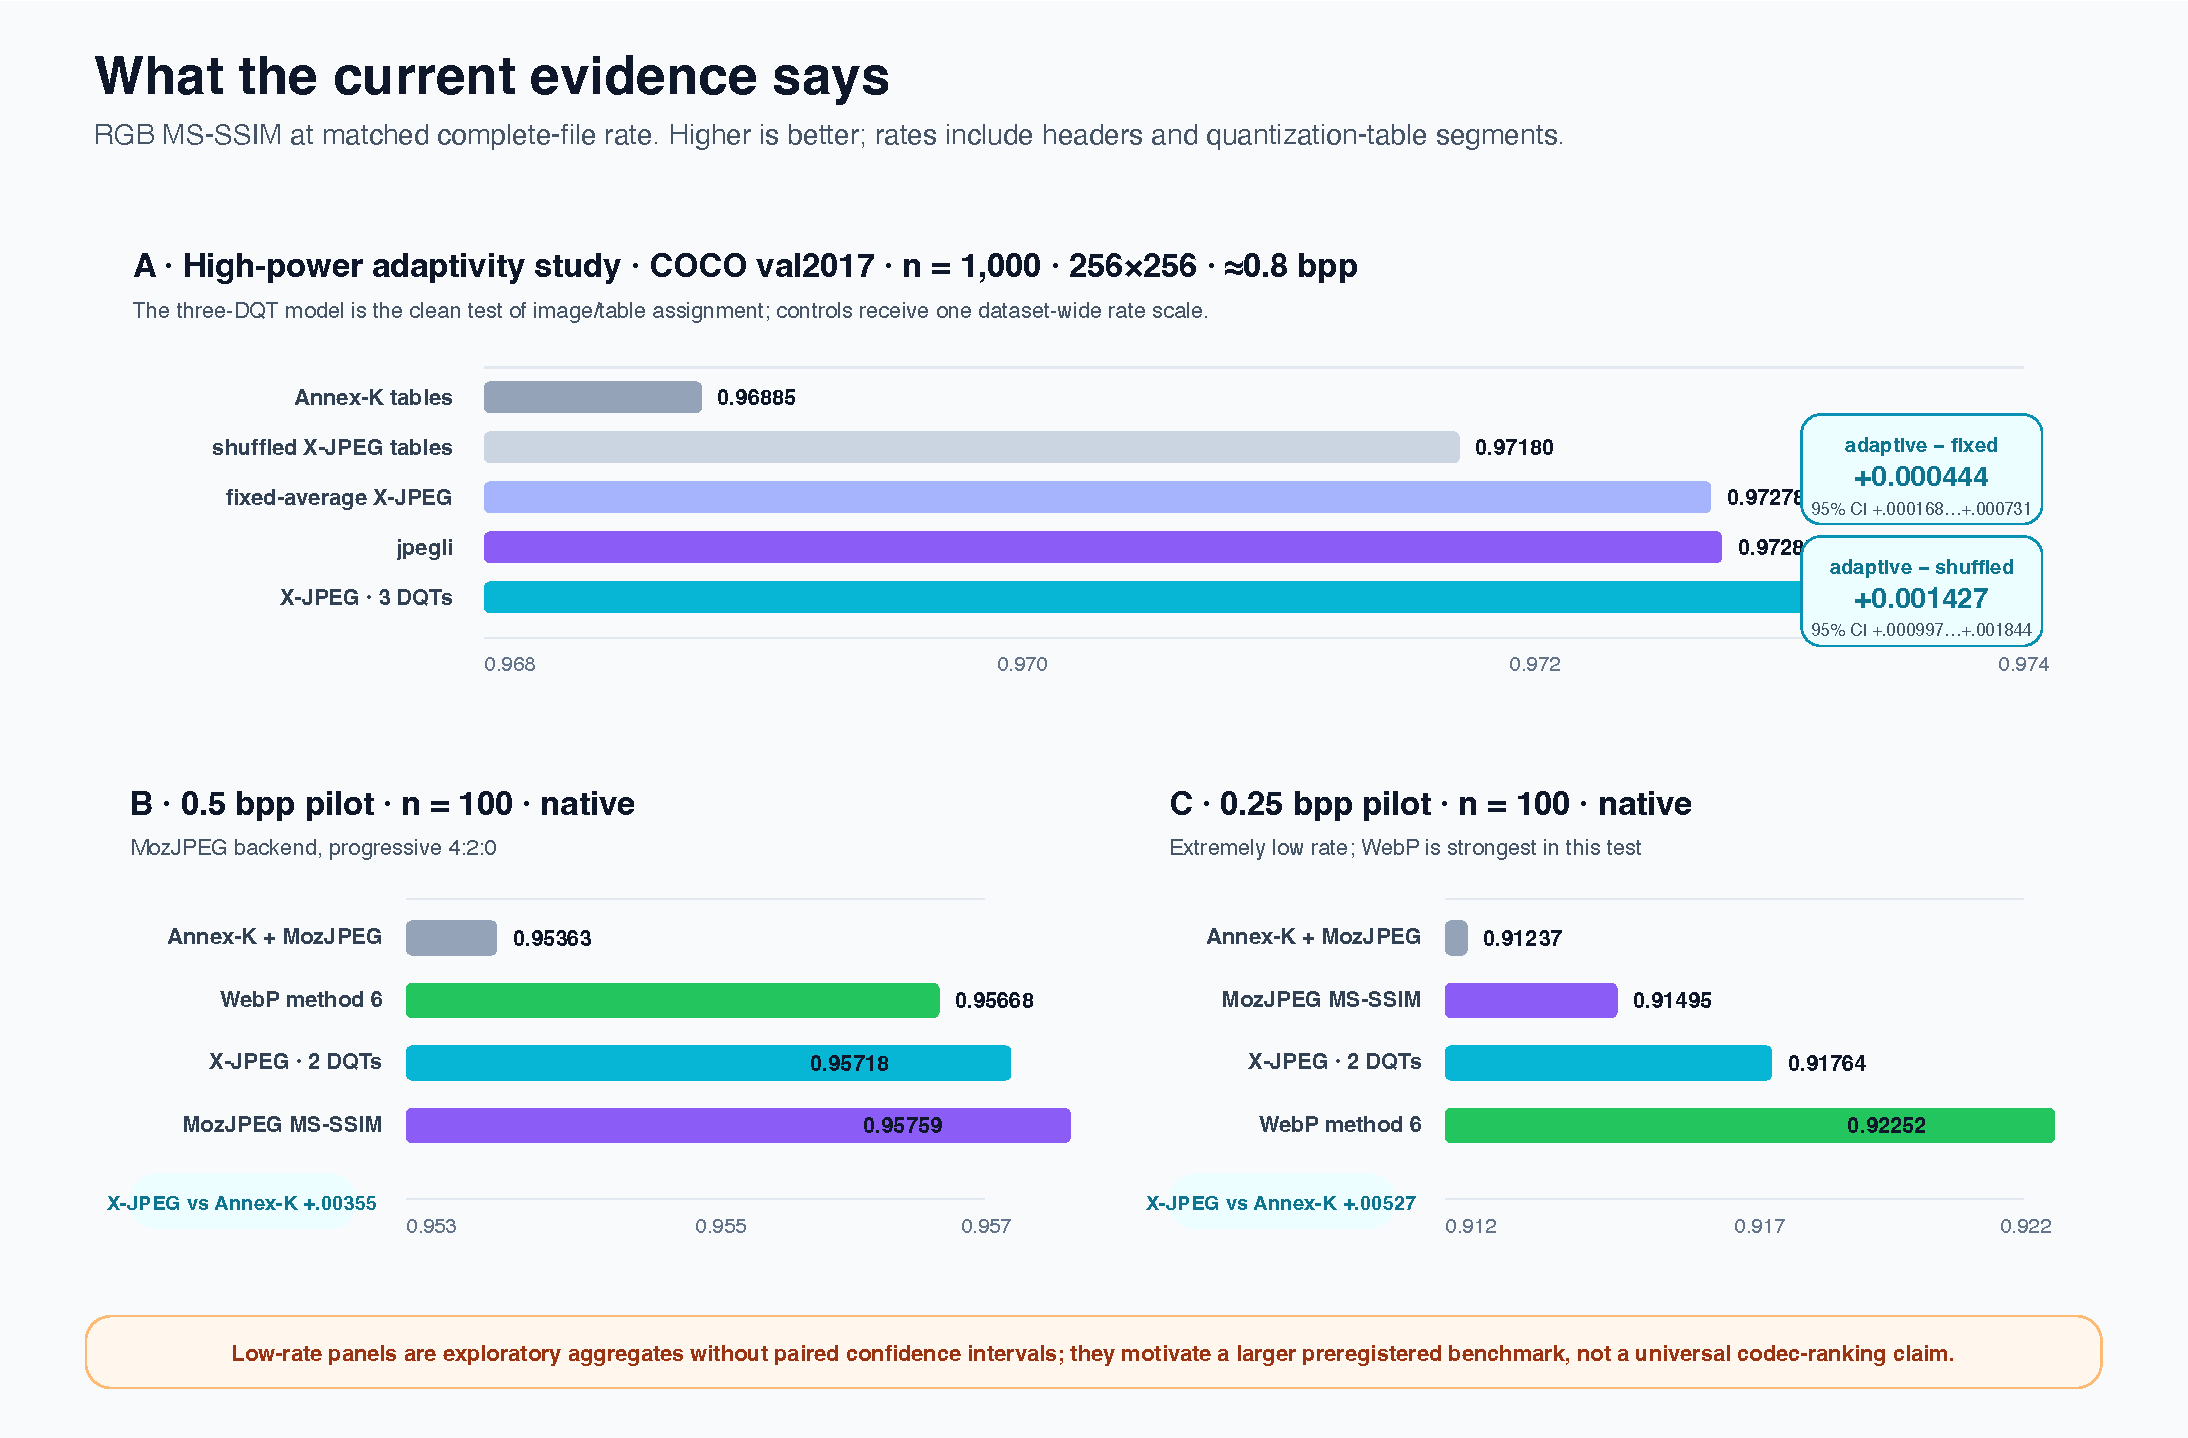
\includegraphics[width=\textwidth]{figures/pdf/05-evidence.pdf}
  \caption{Evidence summary. Adaptivity uses 1,000 images and paired bootstrap intervals. Low-rate panels use 100 images and are exploratory.}
  \label{fig:evidence}
\end{figure*}

\section{Ablations}

\paragraph{Native DCT statistics.}
Frequency-aligned full-image statistics improve the direct libjpeg path over equally trained no-stat controls by about +0.00054 RGB \msssim{} at 0.8 bpp and +0.00080 at 0.5 bpp. On COCO-val-1000 near 0.5 bpp, adaptive minus fixed is +0.000564 (95\% CI +0.000118--+0.001004). Learned statistic gains move materially away from initialization.

\paragraph{Soft table entropy.}
Keeping weight 0.01 versus turning it off gives numerically indistinguishable product results, consistent with literal DQT storage. It remains available for historical reconstruction; the finalist uses zero.

\paragraph{Mirror decoder and initialization.}
The autoencoder loss is unnecessary in the selected product continuation. A small nonzero bottleneck-head initialization and explicit wrong-image controls are more important to avoiding global-table collapse. The decoder is not shipped.

\paragraph{Width.}
A controlled two-times-width run did not improve the frontier within its budget. More parameters do not automatically produce better tables; optimization and input evidence matter.

\paragraph{Third-DQT overhead.}
Three outputs preserve the full predictor, but a third DQT can hurt small files. Averaging chroma only at emission frequently improves complete-file performance by saving roughly 65 bytes.

\section{Limitations}

\begin{enumerate}
  \item The model is optimized primarily for RGB \msssim{} with a luma guard; it can lead on RGB while trailing on luma.
  \item Standard DQT compatibility restricts allocation to one table per component/image, not block-level adaptation.
  \item The Laplace rate proxy omits material JPEG coding details; real-file validation remains mandatory.
  \item Training/evaluation are dominated by natural COCO photographs. Medical, synthetic, text-heavy, scanned, and adversarial imagery are uncharacterized.
  \item The 0.5/0.25-bpp comparison has 100 images and no paired intervals.
  \item On an Intel Xeon Platinum 8480+, table prediction takes 10.4 ms median / 13.0 ms p95 on a 50-image subset (median 0.273 MP); stock JPEG adds 1.5 / 2.5 ms. Other hardware requires measurement.
  \item Encoding requires an 8.4 MB model and current PyTorch runtime, though decoding is model-free.
  \item Per-image target-rate search performs multiple encodes and must not be confused with evidence of adaptivity.
  \item Final-checkpoint seed variability remains unmeasured.
\end{enumerate}

\section{Reproducibility}

Version 0.1.0 is MIT licensed at \url{https://github.com/trinity-cloud/x-jpeg}; the model is at \url{https://huggingface.co/migtissera/x-jpeg}; installation is \texttt{pip install xjpeg}. The output opens with an ordinary JPEG decoder.

The released Safetensors SHA-256 is
\begin{quote}\ttfamily\footnotesize
823a305b9cdf6d16e2296644d88a343d\\
fc68621fa8e3d4b3c0125772c50b92e8
\end{quote}
and its source encoder checkpoint SHA-256 is
\begin{quote}\ttfamily\footnotesize
5878df379ff23dbfa1c1e753d0a70d2b\\
131e4625cc20be2b61fc882789304219.
\end{quote}
The current checkpoint was trained in 2026 from the open PyTorch implementation. No prior private model weights are present in the package; every empirical claim here refers to the released artifact.

\section{Conclusion}

\xjpeg{} treats a mature file format as a platform rather than an obstacle. A network makes an encoder decision JPEG already represents: which frequencies and components deserve bits in this image. The decoder remains unchanged.

The central result is not merely a gain over a standard table. Correctly pairing the released model's table with its source beats both fixed-average and wrong-image tables on 1,000 held-out samples with paired intervals above zero. This establishes genuine image-conditioned utility inside a standard JPEG bitstream. Low-rate pilots further suggest that benefit over fixed JPEG tables grows as bits become scarce, while showing that WebP remains ahead at 0.25 bpp in the present comparison.

The next research step is a preregistered multi-dataset low-rate study with paired uncertainty, visual examples, and encode-time accounting. The immediate product result already exists: \xjpeg{} emits files the world can decode today.

\balance
\bibliographystyle{unsrt}
{\small\bibliography{references}}

\end{document}
